\documentclass{article}
\usepackage{graphicx} % Required for inserting images
\usepackage[section]{placeins}
\usepackage{float}
\usepackage{amsmath,amsthm}
\usepackage[margin=1in]{geometry}
\usepackage{fancyhdr}
\usepackage{enumitem}
\usepackage{graphicx}
\usepackage{amsmath}
\usepackage{amssymb}
\usepackage{algorithm}
\usepackage{algorithmic}
\usepackage{subfig}


\title{Assignment 2}
\date{November 14, 2023}
\author{
  Ravi Raghavan\\
  \texttt{rr1133}
  \and
  Michelle Han\\
  \texttt{mmh255}
}
\begin{document}

%%%%%%%%% PART 1 %%%%%%%%%%%%%%%%%%%
\maketitle
\section{Motion Planning for a 2-link Planar Arm}
% SECTION 1.1
\subsection{Sampling Random Collision-Free Configurations}
% SECTION 1.1 FIGURES
\begin{figure}[h!]
     \begin{minipage}{0.48\textwidth}
    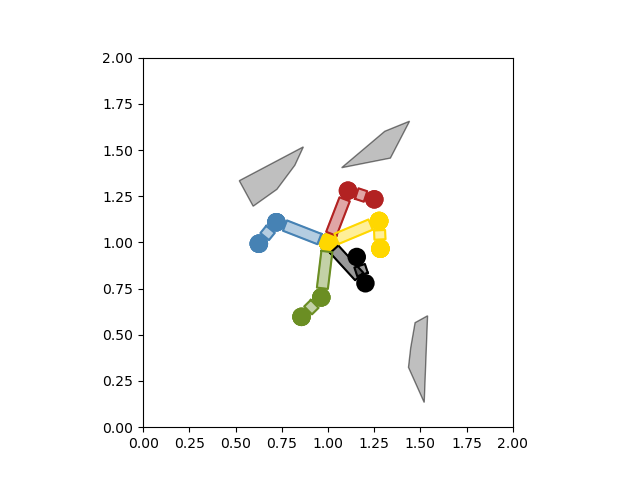
\includegraphics[width=\linewidth]{p1.1.1.png}
    \caption{Provided environment}
  \end{minipage}\hfill
  \begin{minipage}{0.48\textwidth}
    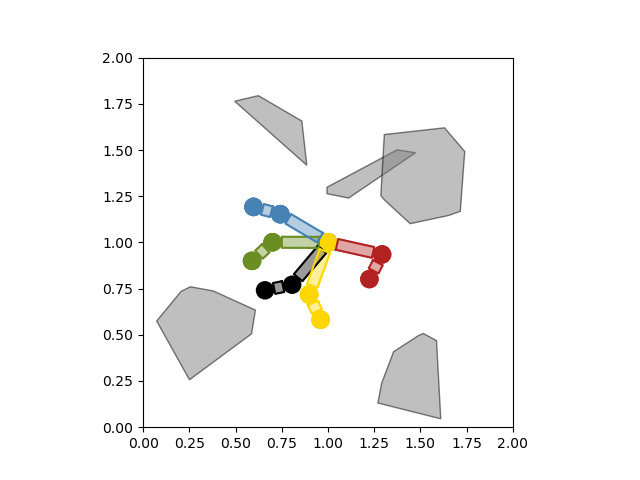
\includegraphics[width=\linewidth]{p1.1.2.png}
    \caption{Assignment 1 environment}
  \end{minipage}\hfill
\end{figure}
% SECTION 1.2
\subsection{Nearest Neighbors}
To find the nearest neighbors, the distance was measured using the end-effector positions. For implementation, forward kinematics was used to determine the coordinates of the end-effectors and the Eucliean distance was calculated from the coordinates.
% SECTION 1.2 FIGURES
\begin{figure}[htbp]
  \centering
  \begin{minipage}{0.45\textwidth}
    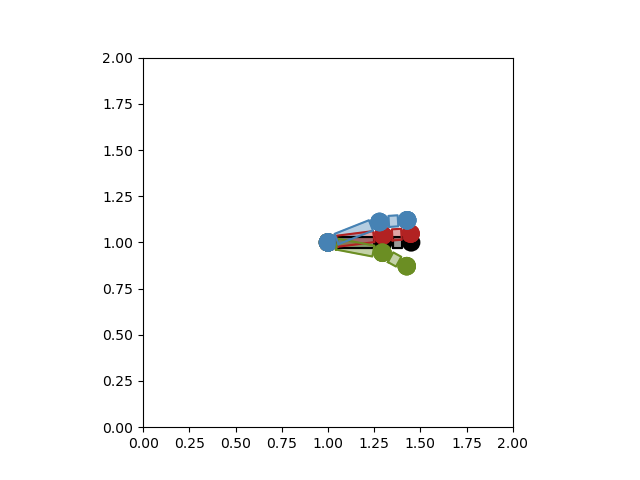
\includegraphics[width=\linewidth]{p1.2.1.png}
    \caption{target = [0,0], k=3}
  \end{minipage}\hfill
  \begin{minipage}{0.45\textwidth}
    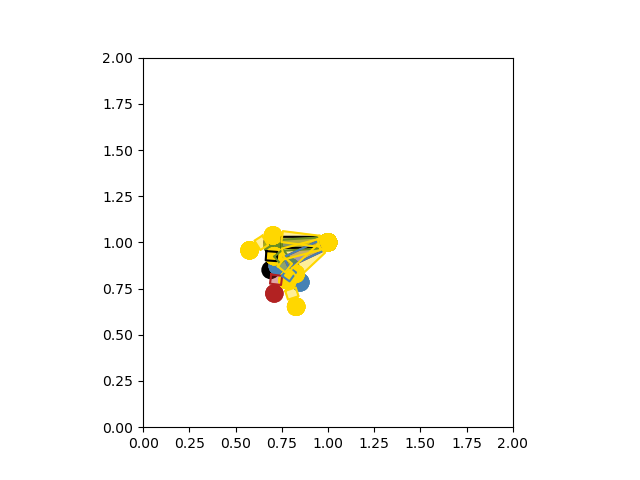
\includegraphics[width=\linewidth]{p1.2.2.png}
    \caption{target = [3.14,1.5], k=6}
  \end{minipage}
  \begin{minipage}{0.45\textwidth}
    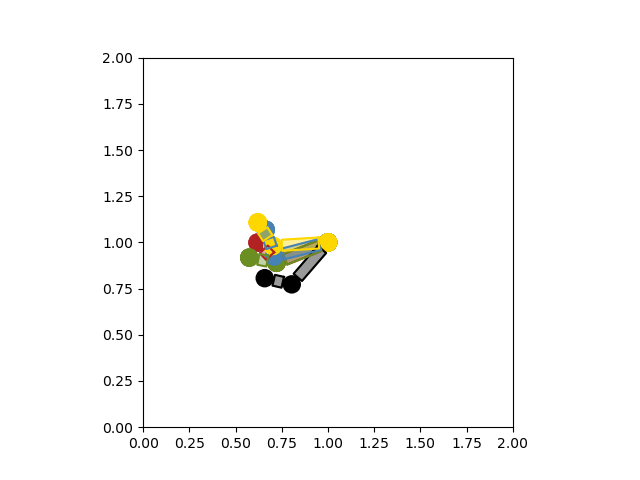
\includegraphics[width=\linewidth]{p1.2.3.png}
    \caption{target = [4,5.2], k=4}
  \end{minipage}\hfill
  \begin{minipage}{0.45\textwidth}
    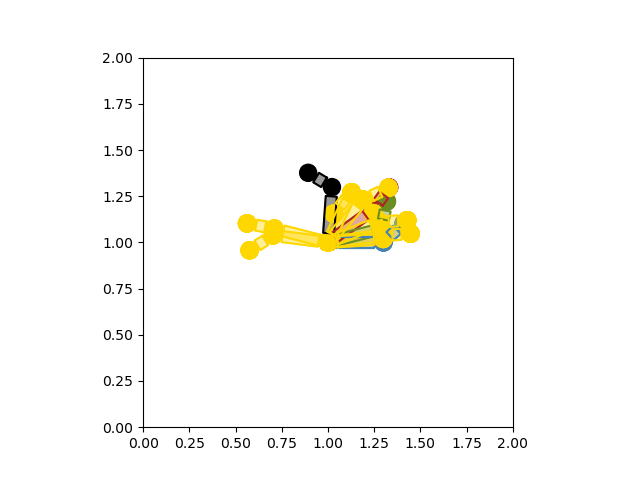
\includegraphics[width=\linewidth]{p1.2.4.png}
    \caption{target = [1.5,1.1], k=10}
  \end{minipage}
   \begin{minipage}{0.45\textwidth}
    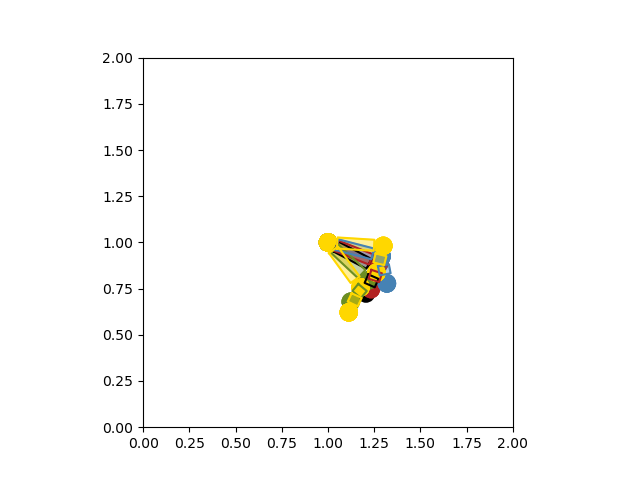
\includegraphics[width=\linewidth]{p1.2.5.png}
    \caption{target = [5.8,-1.5], k=5}
  \end{minipage}
\end{figure}
\subsubsection{With Linear Search Approach}
To implement the Linear Search,
% SECTION 1.2 -> EXTRA CREDIT
\subsubsection{With KD-Tree Search Approach}
To implement the KD-Tree Search,
\subsubsection{Search Comparison}
To compare running times between linear search and kd-tree search, the map used was arm\_polygons.npy and the target was [3.14, 0]. When comparing the running time as the number of configurations increased, the k nearest neighbors was set to 3. When comparing the running time as the number of neighbors increased, the number of random configurations was 100. 
\begin{figure}[]
  \centering
    \includegraphics[width=\linewidth]{comp_k.png}
    \caption{Running time vs. number of nearest neighbors}
    \includegraphics[width=\linewidth]{comp_configs.png}
    \caption{Running time vs. number of configurations}
\end{figure}
\subsubsection{Visualizations}
\begin{figure}[htbp]
  \centering
  \begin{minipage}{0.45\textwidth}
    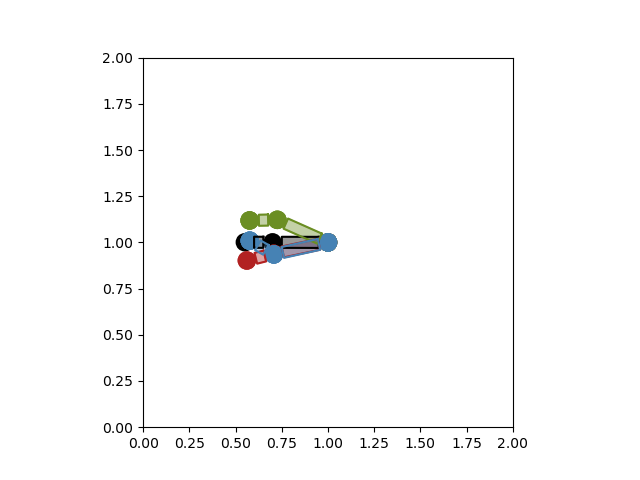
\includegraphics[width=\linewidth]{p1.2.ec100.png}
    \caption{}
  \end{minipage}\hfill
  \begin{minipage}{0.45\textwidth}
    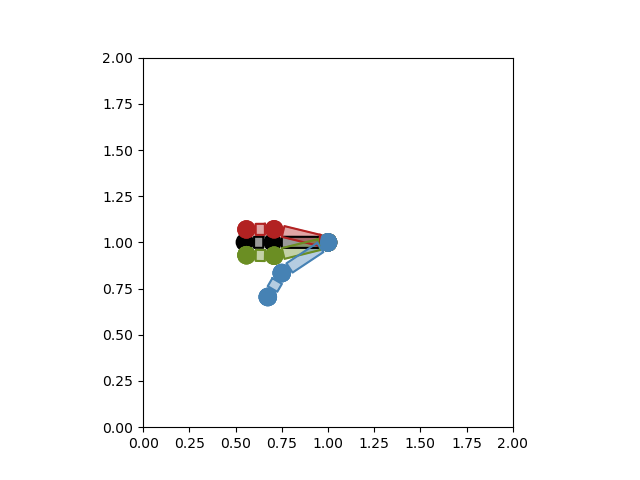
\includegraphics[width=\linewidth]{p1.2.ec500.png}
    \caption{}
  \end{minipage}
  \begin{minipage}{0.45\textwidth}
    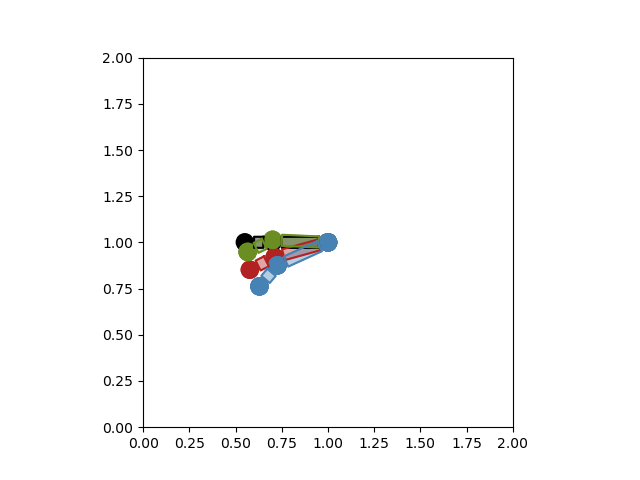
\includegraphics[width=\linewidth]{p1.2.ec1000.png}
    \caption{}
  \end{minipage}\hfill
  \begin{minipage}{0.45\textwidth}
    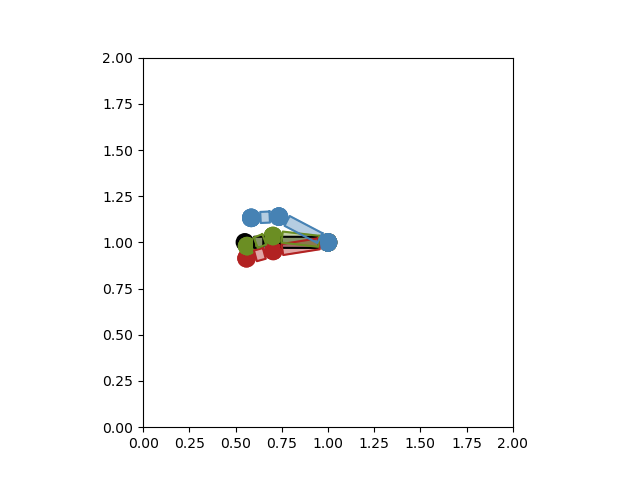
\includegraphics[width=\linewidth]{p1.2.ec2000.png}
    \caption{}
  \end{minipage}
\end{figure}
\begin{figure}[htbp]
  \centering
  \begin{minipage}{0.45\textwidth}
    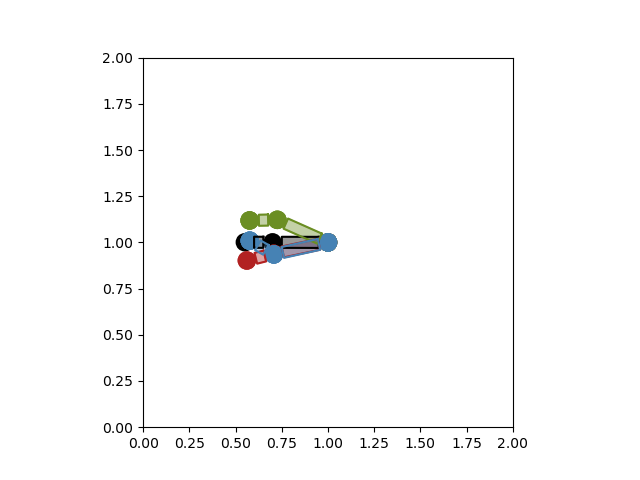
\includegraphics[width=\linewidth]{p1.2.ec3n.png}
    \caption{}
  \end{minipage}\hfill
  \begin{minipage}{0.45\textwidth}
    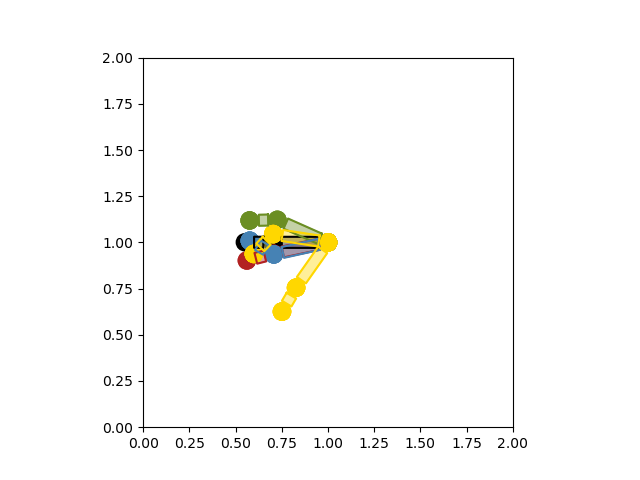
\includegraphics[width=\linewidth]{p1.2.ec5n.png}
    \caption{}
  \end{minipage}
  \begin{minipage}{0.45\textwidth}
    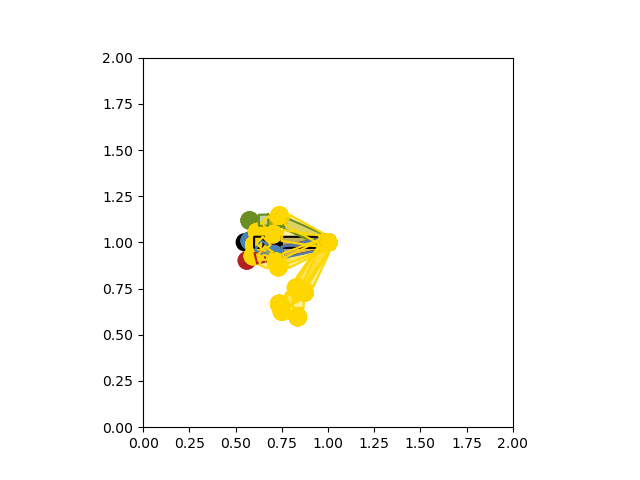
\includegraphics[width=\linewidth]{p1.2.ec10n.png}
    \caption{}
  \end{minipage}\hfill
  \begin{minipage}{0.45\textwidth}
    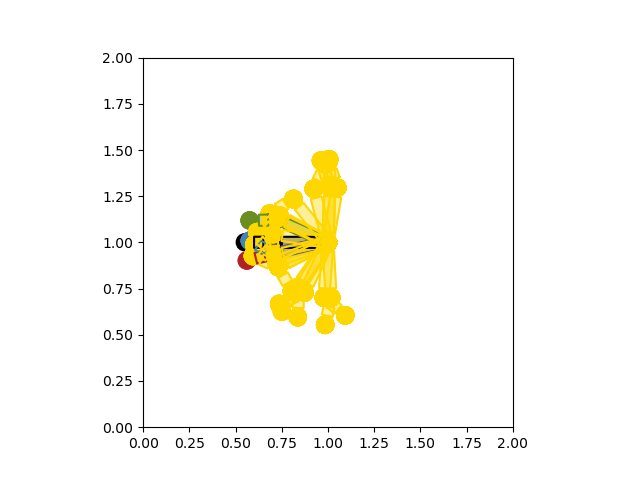
\includegraphics[width=\linewidth]{p1.2.ec20n.png}
    \caption{}
  \end{minipage}
\end{figure}
% SECTION 1.3
\subsection{Interpolation Along the Straight Line in the C-Space}
describe implementation and resulting visualizations
% SECTION 1.4
\subsection{RRT Implementation}
explain RRT implementation
how did i decide to add an edge to tree
% SECTION 1.5
\subsection{PRM Implementation}
explain PRM implementation
% SECTION 1.6 -> EXTRA CREDIT
\subsubsection{PRM*}
explain PRMstar and how i changed PRM
\subsubsection{Planner Comparison}
%%%%%%%%% PART 2 %%%%%%%%%%%%%%%%%%%
\maketitle
\section{Motion Planning for a Rigid Body in 2D}
% SECTION 2.1
\subsection{Sampling Random Collision-Free Configurations}
\begin{figure}[h!]
	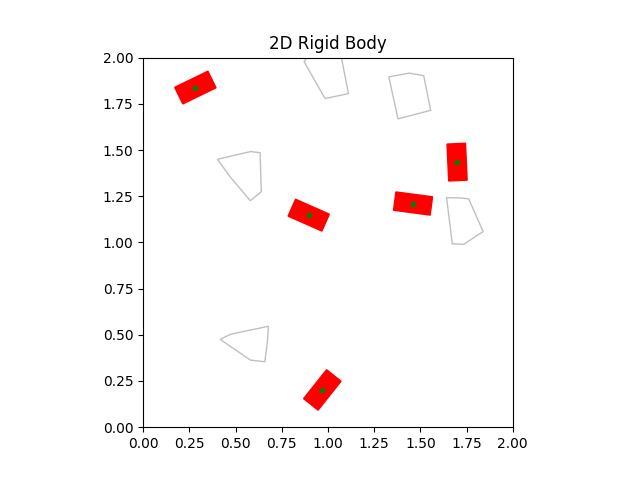
\includegraphics[width= 0.9 \linewidth]{P2_collision_free(1).png}
	\centering
	\caption{Collision-Free Sampling for Environment 1}
	\label{P2_collision_free(1).png}
\end{figure}

Shown in the image above is a plot of the environment with 5 random collision-free configurations of the Rigid Body. For each configuration, the green dot represents the geometric center of the rigid body when it is in that configuration. 

\newpage 
\begin{figure}[h!]
	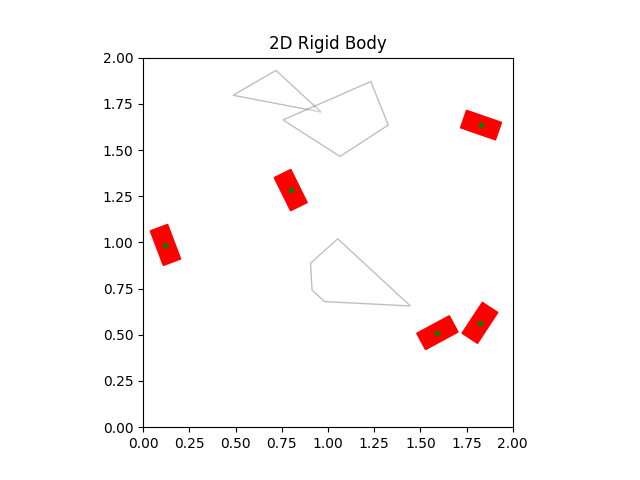
\includegraphics[width= 0.9 \linewidth]{P2_collision_free(2).png}
	\centering
	\caption{Collision-Free Sampling for Environment 2}
	\label{P2_collision_free(2).png}
\end{figure}
Shown in the image above is a plot of the environment with 5 random collision-free configurations of the Rigid Body. For each configuration, the green dot represents the geometric center of the rigid body when it is in that configuration. 

\newpage 
\begin{figure}[h!]
	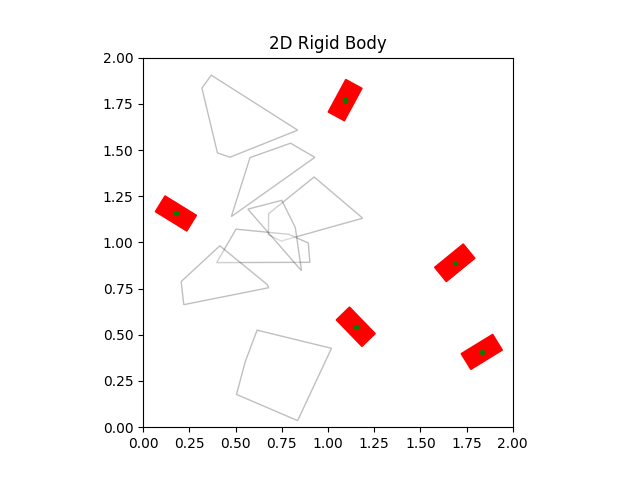
\includegraphics[width= 0.9 \linewidth]{P2_collision_free(3).png}
	\centering
	\caption{Collision-Free Sampling for Environment 3}
	\label{P2_collision_free(3).png}
\end{figure}
Shown in the image above is a plot of the environment with 5 random collision-free configurations of the Rigid Body. For each configuration, the green dot represents the geometric center of the rigid body when it is in that configuration. 



\newpage 
\subsubsection{Analysis}
For Problem 2, we know that our configuration $q$ for the 2D Rigid Body can be represented as $(x, y, \theta)$ where $(x, y)$ are the coordinates of the rigid body's geometric center and $\theta$ is the degree of rotation of the rigid body with respect to its center. 

Hence, to obtain 5 samples of random collision-free configurations, I followed the following basic steps 5 times! : 
\begin{itemize}
    \item I sampled $x_{rand}$ uniformly from the range $(0, 2)$, I sampled $y_{rand}$ uniformly from the range $(0, 2)$, and I sampled $\theta_{rand}$ uniformly from the range $(-\pi, \pi)$
    \item The configuration I obtained was $(x_{rand}, y_{rand}, \theta_{rand})$
    \item To determine whether this configuration was in the Free Space of the Configuration Space, I converted the configuration to workspace coordinates and applied collision checking(same algorithms I used in Assignment 1)
    \item If the configuration was in the Free Space of the Configuration Space, I kept it
\end{itemize}

\subsubsection{Collision Detection Review}
To implement collision detection, my methodology can be broken down into two major portions. Let's say we are trying to detect if Polygon P and Q collide. The first thing I did was to construct bounding boxes around each polygon. Essentially, a bounding box for a polygon is akin to drawing a rectangle around the polygon that covers all its corners \newline 

Once the bounding boxes are constructed, when checking for collision, the first thing I check to see is if the bounding boxes for P and Q intersect. If no intersection is detected, I simply return False to indicate that there is NO collision. \newline 

However, if there is a collision detected between the bounding boxes of P and Q, I need to verify this collision. To do this verification, I use the Separating Axis Theorem(SAT). \newline 

Essentially, the main principle behind the Separating Axis Theorem is as follows. If a line/axis exists such that the projections of two polygons onto this line don't overlap, then the polygons don't collide. \newline 

For each edge of both polygons, I computed the normal vector to that edge. Then, I projected each polygon onto that normal vector. If there was a gap in the projections(i.e. there was no overlap in the projections), then I could conclude that there was NO intersection between the two polygons. 

If there was no such gap, I would have to keep continuing this process until I found a normal vector where there was a gap in the projections of the polygons onto this vector. 

At the end of the process, if I did not find any such gap of the projections onto any of the normal vectors, I could conclude that there was a collision between the polygons 

% SECTION 2.2
\newpage 
\subsection{Nearest Neighbors with Linear Search Approach}
\begin{figure}[h!]
	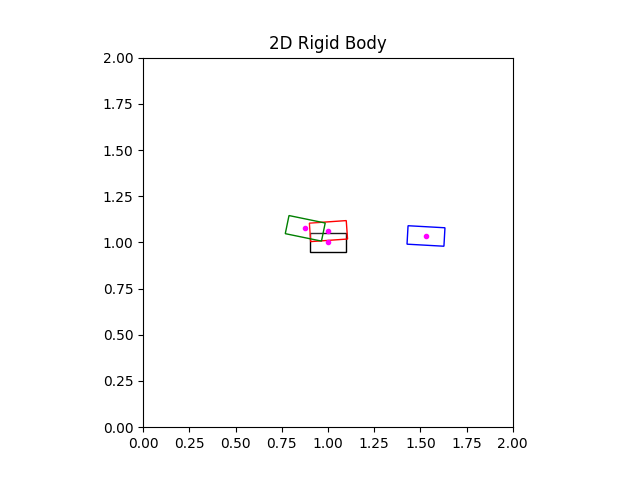
\includegraphics[width= 0.9 \linewidth]{P2_NearestNeighbor(1).png}
	\centering
	\caption{Nearest Neighbors(1)}
	\label{P2_NearestNeighbor(1).png}
\end{figure}

\underline{Program Input}: Target Configuration was $[1, 1, 0]$, number of nearest neighbors was 3, and the input list was specified by rigid$\_$configs.npy
\newpage 
\begin{figure}[h!]
	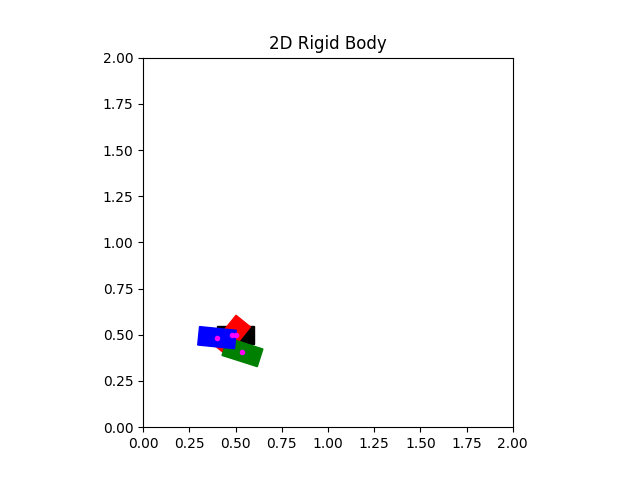
\includegraphics[width= 0.9 \linewidth]{P2_NearestNeighbor(2).png}
	\centering
	\caption{Nearest Neighbors(2)}
	\label{P2_NearestNeighbor(2).png}
\end{figure}

\underline{Program Input}: Target Configuration was $[0.5, 0.5, 0]$, number of nearest neighbors was 3, and the input list was specified by rigid$\_$configs.npy

\newpage 
\begin{figure}[h!]
	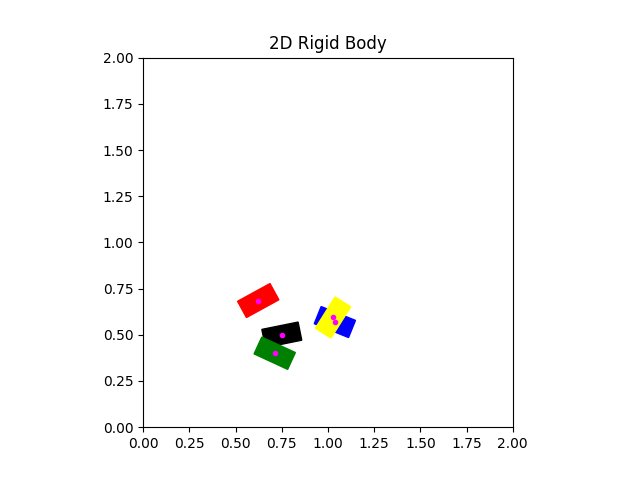
\includegraphics[width= 0.9 \linewidth]{P2_NearestNeighbor(3).png}
	\centering
	\caption{Nearest Neighbors(3)}
	\label{P2_NearestNeighbor(3).png}
\end{figure}

\underline{Program Input}: Target Configuration was $[0.75, 0.5, 0.2]$, number of nearest neighbors was 4, and the input list was specified by rigid$\_$configs.npy

\newpage 
\begin{figure}[h!]
	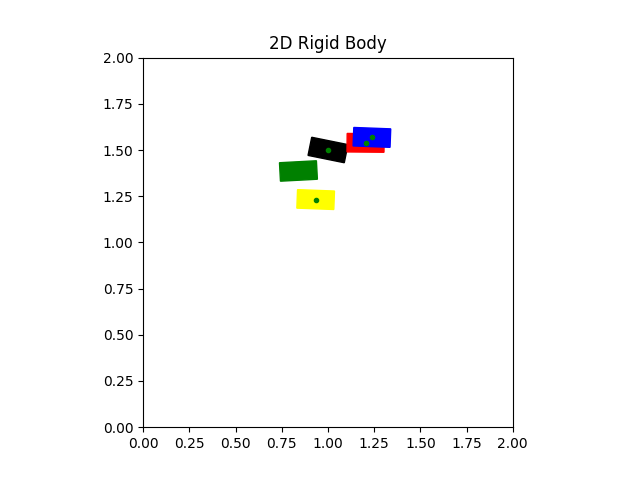
\includegraphics[width= 0.9 \linewidth]{P2_NearestNeighbor(4).png}
	\centering
	\caption{Nearest Neighbors(4)}
	\label{P2_NearestNeighbor(4).png}
\end{figure}

\underline{Program Input}: Target Configuration was $[1, 1.5, -0.2]$, number of nearest neighbors was 4, and the input list was specified by rigid$\_$configs.npy

\newpage
\begin{figure}[h!]
	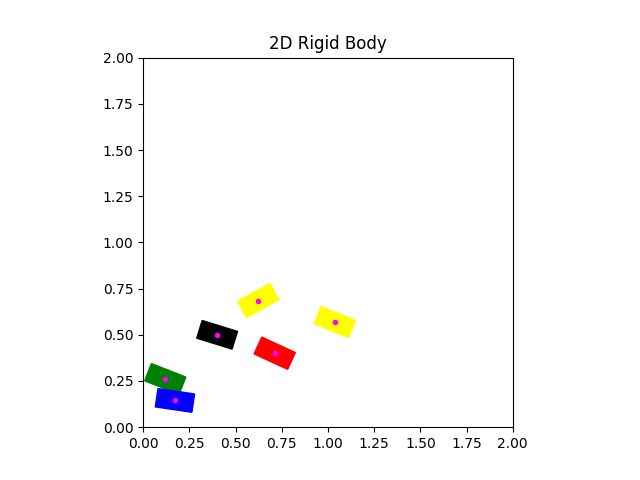
\includegraphics[width= 0.9 \linewidth]{P2_NearestNeighbor(5).png}
	\centering
	\caption{Nearest Neighbors(5)}
	\label{P2_NearestNeighbor(5).png}
\end{figure}

\underline{Program Input}: Target Configuration was $[0.4, 0.5, -0.3]$, number of nearest neighbors was 5, and the input list was specified by rigid$\_$configs.npy

\subsubsection{Analysis}
First, I will explain the distance metric to compute the distance between two configurations and how I went about computing this distance.  \newline 

Distance Metric: $D = \alpha d_t + (1 - \alpha) d_r$ \newline 
where $\alpha = 0.7$, $d_t$ is the Euclidean Distance between two configurations, $d_r$ is the Rotational Distance between two configurations. 

Let's say we have two configurations: $(x_1, y_1, \theta_1)$ and $(x_2, y_2, \theta_2)$, here is how I would go about computing the distance between the two configurations: \newline 

$d_t = \sqrt{(x_2 - x_1)^2 + (y_2 - y_1)^2}$ \newline 

Calculating $d_r$ was also rather straightforward but I had to account for the topology here. The topology, for the 2D Rigid Body, was $SE(2)$. Hence, for $\theta$, the angles can "wrap around" in a circle. 

Hence, To calculate $d_r$, given $\theta_1$ and $\theta_2$, here is a rough algorithm of what I followed


\begin{algorithm}
\caption{Calculation of $d_r$}
\begin{algorithmic}
\STATE Parameters: $theta_1$, $theta_2$

\STATE {$d_r = min(abs( \theta_1 - \theta_2), 2\pi -abs(\theta_1 - \theta_2) )$}

\end{algorithmic}
\end{algorithm}


% SECTION 2.3
\subsection{Interpolation Along the Straight Line in the C-Space}
\subsubsection{Analysis}
Let's say we have two configurations: $(x_1, y_1, \theta_1)$ and $(x_2, y_2, \theta_2)$. To interpolate along the straight line from $(x_1, y_1, \theta_1)$ to  $(x_2, y_2, \theta_2)$, I would connect $(x_1, y_1, \theta_1)$ to  $(x_2, y_2, \theta_2)$ and then divide the line into multiple segments. \newline 

For example, I would divide the line segment from $(x_1, y_1, \theta_1)$ to  $(x_2, y_2, \theta_2)$ into $n$ segments, and animate the rigid body moving along those n segments. 

% SECTION 2.4
\subsection{RRT Implementation}

Let $V$ be the set of vertices of the RRT and $E$ be the set of edges of the RRT. 

\begin{algorithm}
\caption{RRT Algorithm}
\begin{algorithmic} 
\STATE Parameters: $N$ (number of nodes we want to have in our RRT), $q_{start}$(Node to start our RRT From), $q_{goal}$ (Goal Node)

\STATE{$V = V \cup \{ q_{start}\}$}
\STATE i $\rightarrow$ 1

\WHILE{$i < N$}
\STATE {Sample $q_{rand}$ from the free configuration space} 
\STATE {Let $q_{near}$ be the point on the RRT that is closest to $q_{rand}$.}
\STATE {From $q_{near}$, draw a straight line from $q_{near}$ to $q_{rand}$. Make sure to step towards $q_{rand}$ in small steps from $q_{near}$.}
\STATE {If we hit an obstacle, let $q_{steer}$ be the last point we visited on the straight line interpolation with $q_{rand}$ where we didn't collide with an obstacle.}

\IF{A point like $q_{steer}$ could NOT found on the straight line interpolated path from $q_{rand}$ to $q_{}$}
\STATE{Continue to next Iteration}
\ELSE
\STATE{$V = V \cup \{q_{steer\} }$, $E = E \cup \{(q_{rand}, q_{steer})\}$}
\STATE {i $\rightarrow i + 1$ } 
\ENDIF
\ENDWHILE

\IF{$q_{goal} \notin V$}
\STATE{Let $q_{near}$ be the point on the RRT that is closest to $q_{goal}$.}
\STATE{Output the Path from $q_{start}$ to $q_{near}$}

\ENDIF

\end{algorithmic}
\end{algorithm}


% SECTION 2.5
\newpage 
\subsection{PRM Implementation}
Let $V$ be the set of vertices of the PRM and $E$ be the set of edges of the PRM. 


\begin{algorithm}
\caption{PRM Algorithm}
\begin{algorithmic} 
\STATE Parameters: $N$ (number of nodes we want to have in our PRM), 
$k$ (how many neighbors we want to analyze when forming edges)
\STATE i $\rightarrow$ 0
\WHILE {$i < N$}
\STATE {Sample $q_{rand}$ from the free configuration space} 
\STATE {$V = V \cup \{q_{rand\} }$}
\STATE {Let $Q_{neighbors}$ be the $k$ nearest neighbors of $q_{rand}$ out of all the nodes currently in the PRM }

\FOR{$q_{n} \in Q_{neighbors}$}
\IF{There is a collision free path between $q_{n}$ and $q_{rand}$}
\STATE{$E = E \cup \{(q_{n}, q_{rand})\}$}\ENDIF
\ENDFOR
\STATE {i $\rightarrow i + 1$ } 
\ENDWHILE

\end{algorithmic}
\end{algorithm}

\begin{algorithm}
\caption{PRM Query}
\begin{algorithmic}
\STATE Parameters: $q_{start}$(Start Node), $q_{goal}$ (Goal Node), $k$ (how many neighbors we want to analyze when forming edges)

\STATE {Let $Q_{neighbors}$ be the $k$ nearest neighbors of $q_{start}$ out of all the nodes currently in the PRM.}

\FOR{$q_{n} \in Q_{neighbors}$}
\IF{There is a collision free path between $q_{n}$ and $q_{start}$}
\STATE{$E = E \cup \{(q_{n}, q_{start})\}$}\ENDIF
\ENDFOR

\STATE {Let $Q^2_{neighbors}$ be the $k$ nearest neighbors of $q_{goal}$ out of all the nodes currently in the PRM.}

\FOR{$q_{n} \in Q^2_{neighbors}$}
\IF{There is a collision free path between $q_{n}$ and $q_{goal}$}
\STATE{$E = E \cup \{(q_{n}, q_{goal})\}$}\ENDIF
\ENDFOR

\STATE{Run $A^*$ Search Algorithm on the PRM Graph to find a path from $q_{start}$ to $q_{goal}$ in the Configuration space via the nodes on our PRM}

\end{algorithmic}

\end{algorithm}


%%%%%%%%% PART 3 %%%%%%%%%%%%%%%%%%%
\newpage 
\maketitle
\section{Motion Planning for a First-Order Car}
% SECTION 3.1
\subsection{Implementation of Dynamics}
Configurations are defined as such: \newline 
\begin{align}
    q(t) &= \begin{bmatrix}
           x(t) \\
           y(t) \\
           \theta(t)
         \end{bmatrix}
\end{align}

Controls are defined as such: \newline 
\begin{align}
    u(t) &= \begin{bmatrix}
           v(t) \\
           \phi(t)
         \end{bmatrix}
\end{align}

Derivative of Configuration is defined as such: \newline 
\begin{align}
    \dot{q}(t) &= \begin{bmatrix}
           v\cos{\theta(t)} \\
           v\sin{\theta(t)} \\
           \frac{v}{L} \tan{\phi}
         \end{bmatrix}
\end{align}

System Dynamics: \newline 
\begin{align}
    q(t + dt) &= q(t) + \dot{q}(t) dt
\end{align}

Instructions to Control Keyboard Animation: \newline 

\begin{itemize}
    \item Up: Increase Velocity
    \item Down: Decrease Velocity
    \item Right: Increase value of $\phi$
    \item Left: Decrease Value of $\phi$
    \item 'c': Keep Controls the same and move along trajectory
\end{itemize}

% SECTION 3.2
\subsection{Integration of Dynamics}
Given a starting configuration(i.e. $q(0)$) and a constant control (i.e. $\mu$), I was able to perform the integration of the above system dynamic equation to determine the trajectory of the car. 

To achieve this, I would simply set $dt = \Delta t = 0.01$. Then, the system dynamic equation can be rewritten as such: \newline 
\begin{align}
    q(t + \Delta t) &= q(t) + \dot{q}(t) \Delta t
\end{align}

\begin{align}
    q(t + 0.01) &= q(t) + \dot{q}(t) (0.01)
\end{align}

The Initial Value of this equation is 

\begin{align}
    q(0) &= \begin{bmatrix}
           x_0 \\
           y_0 \\
           \theta_0
         \end{bmatrix}
\end{align}

The control is constant and can be denoted as such: 
\begin{align}
    u &= \begin{bmatrix}
           v \\
           \phi
         \end{bmatrix}
\end{align}

To solve for the Derivative of Configuration: \newline 
\begin{align}
    \dot{q}(t) &= \begin{bmatrix}
           v\cos{\theta(t)} \\
           v\sin{\theta(t)} \\
           \frac{v}{L} \tan{\phi}
         \end{bmatrix}
\end{align}

The problem description denotes $L = 0.2$. Now, all the necessary information is needed to solve the equation $q(t + 0.01) = q(t) + \dot{q}(t) (0.01)$ for the value of the configuration at the next time step! 
% SECTION 3.3
\subsection{RRT and Planning with Dynamics}

\begin{algorithm}
\caption{Modified RRT For Non-Holonomic Car}
\begin{algorithmic}
\STATE {Randomly sample configurations $q_{rand}$ and identify the closest node $q_{close}$ on the tree to the random sample $q_{rand}$. Occasionally, the goal configuration will be sampled in order to assist RRT in finding a solution (e.g., 5 \% of the time).} \newline 

\STATE {Instead of trying to connect with an edge the closest node $q_{close}$ to the random sample $q_{rand}$, in this version of RRT, a blossom b of random controls $\{u_1, \ldots , u_b\}$ are sampled.} \newline 

\STATE {For each of the b sampled controls $u_i$, integrate forward in time the dynamics from the closest node $q_{close}$ for the same duration $\Delta T$. This results in b possible new states $\{q_{new}^1, \ldots, q_{new}^b \}$ that are reachable from $q_{close}$. Accept a new state only if the integration of the dynamics for time $\Delta T$ does not result in a collision.} \newline 

\STATE{Check the distance between all the new states $\{q_{new}^1, \ldots, q_{new}^b \}$ to the random sample $q_{rand}$ and identify which state $q_{cn}$ among them is the closest to $q_{rand}$ given the distance metric in this configuration space.}

\STATE{add the edge from $q_{close}$ to $q_{cn}$ and store the corresponding control on the edge.}
\end{algorithmic}
\end{algorithm}

\subsubsection{Experimentation}
To experiment with different design choices, my strategy was to change the value of $b$ and observe the success rate of the RRT Algorithm, the resulting path quality of the path returned by the RRT Algorithm, and the overall computational cost. 

I have run these experiments on various polygonal scenes. For each polygonal scene, I ran 5 trials for different values of $b$(i.e. 1, 3, and 5). For each trial on each value of $b$, I report a tuple $(i, j, k)$ \newline 

$i = 0$ if we could NOT find a successful path from the start to the goal region. $i = 1$ if we could find a successful path from the start to the goal region. \newline 

$j$ is equal to the total path distance as computed by the distance metric in this configuration space \newline 

$k$ is the time required to build the RRT in seconds \newline 

Scene 1: $rigid\_polygons.npy$ \newline 
Scene 2: $p2\_scene1.npy$ \newline 
Scene 3: $p2\_scene8.npy$ \newline 

For each experiment, I ran: \newline 
Scene 1: python car\_2.py --start 0.5 0.25 0 --goal 1.75 1.5 0.0 --map "rigid\_polygons.npy" \newline 

Scene 2: python car\_2.py --start 0.5 0.25 0 --goal 1.75 1.5 0.0 --map "p2\_scene1.npy" \newline

Scene 3: python car\_2.py --start 0.25 0.25 -3 --goal 1.2 0.75 0.25 --map "p2\_scene1.npy" \newline


Another thing to note is that, since RRT is probabilistically complete, if we let RRT run with no limit on the number of iterations, it will eventually find a solution(i.e. a path from start to the goal vertex). However, to compare whether a solution can be found across different values of $b$, I wanted to put a maximum limit on the number of iterations we run. I set the maximum limit for the number of iterations as 10000 
 
\begin{table}
  \centering
\begin{tabular}{|c|c|c|c|}
  \hline
  Trial \# & b = 1 & b = 3 & b = 5 \\
  \hline
  1 & (1,8.62,105) & (1,4.87,131) & (1,6.32,14) \\
  2 & (1,7.81,92) & (1,7.37,67) & (1,5.58,147) \\
  3 & (1,9.39,261) & (1,3.77,68) & (1,5.59,176) \\
  4 & (1,4.97,219) & (1,5.81,52) & (1,3.44,21) \\
  5 & (1,6.71,43) & (1,8.81,321) & (1,4.45,104) \\
  Avg & (1, 7.5, 144) & (1, 6.126, 127.8) & (1, 5.076, 92.4)\\
  \hline
\end{tabular} 
\caption{Table for Scene 1}
  \label{tab:mytable}
\end{table}

\begin{table}
  \centering
\begin{tabular}{|c|c|c|c|}
  \hline
  Trial \# & b = 1 & b = 3 & b = 5 \\
  \hline
  1 & (1, 6.83, 261) & (1, 5.47, 61) & (1, 12.57, 574) \\
  2 & (1, 8.63, 559) & (1, 6.19, 46) & (1, 8.60, 128) \\
  3 & (1, 11.99, 267) & (1, 4.43, 3) & (1, 8.13, 125) \\
  4 & (1, 9.11, 1256) & (1, 8.36, 163) & (1, 7.78, 282) \\
  5 & (1, 6.84, 102) & (1, 7.89, 46) & (1, 7.40, 86) \\
  Avg & (1, 8.68, 489) & (1, 6.468, 63.8) & (a, 8.896, 239) \\
  \hline
\end{tabular} 
\caption{Table for Scene 2}
  \label{tab:mytable}
\end{table}

\begin{table}
  \centering
\begin{tabular}{|c|c|c|c|}
  \hline
  Trial \# & b = 1 & b = 3 & b = 5 \\
  \hline
  1 & (1, 8.78, 232) & (1, 3.95, 150) & (1, 11.13, 186) \\
  2 & (1, 3.82, 135) & (1, 7.56, 184) & (1, 6.32, 9) \\
  3 & (1, 3.90, 182) & (1, 7, 264) & (1, 2.99, 239) \\
  4 & (1, 8.05, 144) & (1, 6.76, 128) & (1, 3.65, 16) \\
  5 & (1, 6.61, 156) & (1, 3.56, 31) & (1, 3.25, 281) \\
  Avg & (1, 6.232, 169.8) & (1, 5.766, 151.4) & (1, 5.468, 146.2) \\
  \hline
\end{tabular} 
\caption{Table for Scene 3}
  \label{tab:mytable}
\end{table}

\newpage 
\subsubsection{Scene 1 Analysis}

\textbf{\underline{Impact on RRT Build Time}} \newline

Based on my analysis for Scene 1, the time taken to construct the RRT seems to decrease as I increase the value of $b$. Increasing the value of $b$ enables me to sample more controls during each iteration of the RRT. \newline 

An important thing to keep in mind is that we sample the goal node $5\%$ of the time. For $I$ iterations of RRT, the expected number of times we sample the goal node is $0.05 * I$. When we sample the goal node, due to the fact that we sample more controls as $b$ increases, we are more likely to add a node to the RRT that is closer to the goal node. Hence, as $b$ increases, we are likely to get to the goal region a lot quicker. \newline 


\textbf{\underline{Impact on Path Distance}} \newline

Based on my analysis for Scene 1, the path distance seems to decrease as I increase the value of $b$. Increasing the value of $b$ enables me to sample more controls during each iteration of the RRT. Sampling more controls would allow the RRT Algorithm to explore more areas of the free Configuration Space and, thus, find shorter paths to the goal region \newline 


\textbf{\underline{Impact on Success Rate}} \newline
My experiments show that my RRT Implementation was always successful in finding a path. This showed that 10000 iterations, as a max threshold, was sufficient in letting my RRT Algorithm converge to a solution

\subsubsection{Scene 2 Analysis}

\textbf{\underline{Impact on RRT Build Time}} \newline
Based on my analysis for Scene 2, the time taken to construct the RRT seems to decrease when I increase $b$ from 1 to 3. However, the time taken to construct the RRT increases when I increase $b$ from 3 to 5. Here is my hypothesis for why this is occurring. \newline 

An important thing to keep in mind is that we sample the goal node $5\%$ of the time. For $I$ iterations of RRT, the expected number of times we sample the goal node is $0.05 * I$. When we sample the goal node, due to the fact that we sample more controls as $b$ increases, we are more likely to add a node to the RRT that is closer to the goal node. Hence, as $b$ increases, we are likely to get to the goal region a lot quicker. \newline 

However, when we increase $b$ past a certain point, due to the fact that Scene 2 is rather sparse(i.e. has a few polygonal obstacles) when compared to Scene 1, sampling too many controls may lead us to consider far too many potential directions. Furthermore, since the free space is much bigger, we must consider the Voronoi Bias of the RRT. \newline 

For a recap, here is the definition of the Voronoi Bias of the RRT: Voronoi Bias refers to the fact that the probability of a tree node being selected as the “closest” tree node is proportional to the volume of its Voronoi Region. Our Search is biased towards those nodes with the largest Voronoi Regions(i.e. Unexplored regions of the configuration space)  \newline 

Hence, since RRT is more biased towards the nodes with the largest Voronoi Regions and since our Scene is more sparse(i.e. less polygonal obstacles and bigger free space), we may have the situation where our RRT is exploring regions of the free space that is away from the goal. \newline 

This, in my opinion, would explain the increase in RRT Build Time when $b$ was increased from 3 to 5 \newline 

\textbf{\underline{Impact on Path Distance}} \newline
Based on my analysis for Scene 2, the path distance seems to decrease when I increase $b$ from 1 to 3. However, the path distance increases when I increase $b$ from 3 to 5. Here is my hypothesis for why this is occurring \newline 

Intuitively, when we increase $b$, we would expect the path distance to decrease. Increasing the value of $b$ enables me to sample more controls during each iteration of the RRT. Sampling more controls would allow the RRT Algorithm to explore more areas of the free Configuration Space and, thus, find shorter paths to the goal region \newline 

However, once $b$ crosses a certain threshold, sampling too many controls may lead us to consider far too many potential directions. This may lead the RRT Algorithm astray from the goal node \newline 

\textbf{\underline{Impact on Success Rate}} \newline
My experiments show that my RRT Implementation was always successful in finding a path. This showed that 10000 iterations, as a max threshold, was sufficient in letting my RRT Algorithm converge to a solution

\subsubsection{Scene 3 Analysis}
\textbf{\underline{Impact on RRT Build Time}} \newline

Based on my analysis for Scene 3, the time taken to construct the RRT seems to decrease as I increase the value of $b$. Increasing the value of $b$ enables me to sample more controls during each iteration of the RRT. \newline 

An important thing to keep in mind is that we sample the goal node $5\%$ of the time. For $I$ iterations of RRT, the expected number of times we sample the goal node is $0.05 * I$. When we sample the goal node, due to the fact that we sample more controls as $b$ increases, we are more likely to add a node to the RRT that is closer to the goal node. Hence, as $b$ increases, we are likely to get to the goal region a lot quicker. \newline 


\textbf{\underline{Impact on Path Distance}} \newline

Based on my analysis for Scene 3, the path distance seems to decrease as I increase the value of $b$. Increasing the value of $b$ enables me to sample more controls during each iteration of the RRT. Sampling more controls would allow the RRT Algorithm to explore more areas of the free Configuration Space and, thus, find shorter paths to the goal region \newline 

\textbf{\underline{Impact on Success Rate}} \newline
My experiments show that my RRT Implementation was always successful in finding a path. This showed that 10000 iterations, as a max threshold, was sufficient in letting my RRT Algorithm converge to a solution
\end{document}
